\subsection{From local to distributed filesystems}

\todo{which word to use? distributed filesystem (dfs)?}
\todo{maybe duplicates the introduction}
\todo{is it clear that a san keeps storage for one machine and a dfs shares storage for different users/machines better?}

To offer multiple users and applications a high available access on large filesystems there are different solutions known. 
Files can be stored on local filesystems or may be shared using a Network Attached Storage (NAS) for small businesses or for use at home. While a local filesystem is strongly limited to capacity and multi user access a NAS allows to have a system available for different users. But a NAS is limited for a small number of users and very much limited in world wide file sharing and a secure 24h availability.

A first solution to offer data stores for multiple machines which is actually common in data centers is to setup a Storage Area Network (SAN). This system stores different filesystems for various client machines without being limited to the speed of one physical hard drive. For security reasons it is possible to keep a redundant copy of such a system in a different place and exporting backups, too. But it is not easy to resize that system and not the best solution for sharing the same view of the data to different machines and other machines placed outside of a data centre.

Companies like Facebook were facing these issues and solved them using a distributed filesystem (DFS) \cite{fb-hadoop}. The use of an DFS allows to raise the cluster storage  up to petabytes  \cite{fb-hadoop}. A lot of huge different companies already have decided to use hadoop to store and backup their data  \cite{hadoop-poweredby}. Different algorithms such MapReduce are used to share limitations of cpu power and storage between clustered nodes \cite{dean2008mapreduce}. Further it is easy to raise the number of nodes which makes it highly flexible to use. Only the effort in administration will raise caused on the number of heterogeneous machines.

For cases such as downloading huge files like operating system images it is important to find strategies for reducing traffic by only updating changed parts of such files, named random write. Different interesting questions are about creating snapshots or creating and applying backups where Google was focusing on for their own filesystem implementation \cite{ghemawat2003google}.

Similar functionalities are available through the replacement of fibre channel by  Internet Small Computer System Interface (iSCSI) for SAN. But the use of such a system limits to one manufacturer. Maybe that is one of the main reasons which makes distributed filesystems so popular.

\subsection{Introduction of Apache Hadoop}

The Distributed Filesystem (DFS) should be used to connect cloud storage with a client machine as being local storage as shown in figure~\ref{fig:dfs_example}. To mount the network storage as being local a client program must run on the client machine. By using the DFS it will remove local limitations on Storage while offering a given QoS for bandwidth and multiuser support.

\todo{create a simplified copy in a better fitting style}

\begin{figure}
	\centering
	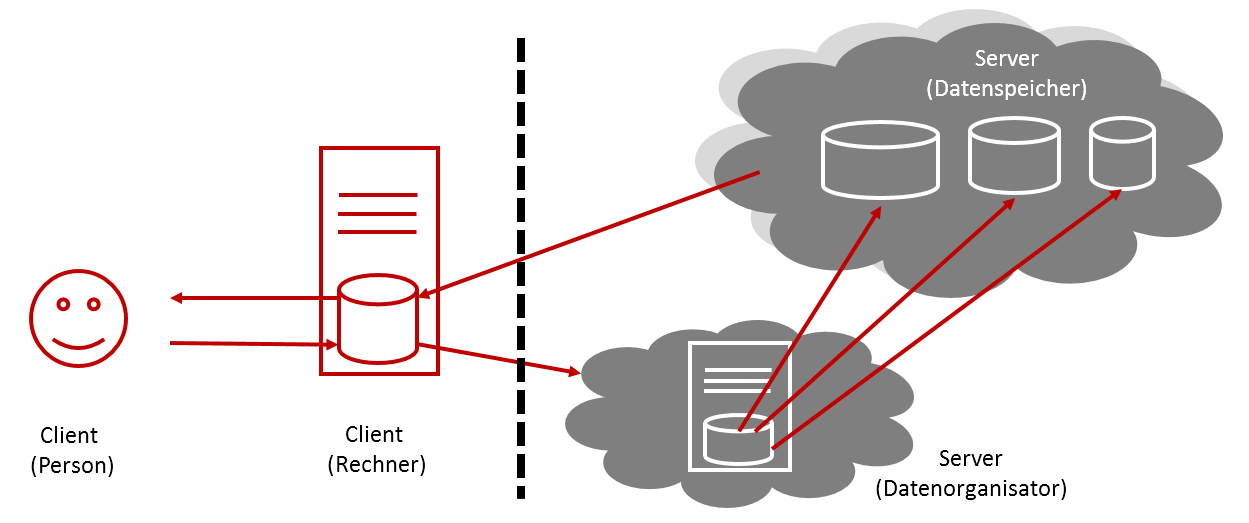
\includegraphics[width=1\linewidth]{img/dfs_example.png}
	\caption{Basic idea of mounting a distributed filesystem}
	\label{fig:dfs_example}
\end{figure}

A research of known DFS brought us the choice between GlusterFS and Apache Hadoop.

GlusterFS is developed by Red Hat Inc. and written in C. Hadoop is part of Apache and written in Java.

Both are open souce and can easily be extended by our own plugins. In addition, both offer a very active community and therefore a steady development. The support of Java was the main reason for the decision for Hadoop.

\todo{move client information to this chapter???}

\subsection{Hadoop setup}

By creating a small cluster in the tubit data centre the power consumption used by system itself and during performing user actions like up- and downloading files is analyzed. For the test system the DFS Apache Hadoop\textsuperscript{\textregistered} is used due to the idea having an DFS running on heterogeneous systems from different hardware and operating systems based on Java. 

Hadoop consists of two main parts. A name server that keeps the logical view of the filesystem and a various number of datanodes which keep the files organized in blocks of a fixed length. Multiple datanodes can be used to raise the available storage amount or to keep multiple replicas of files in different locations for security reasons or to share power between different machines. 

The datanodes were placed on the physical machines of the test system, \textit{Asok05} and the \textit{office pc}. Both are different in power consumption and maximum bandwidth. A connection to the namenode which is placed on the virtual machine was realized through a software defined network which is described in chapter\ref{sec:sdn}.

To assign network traffic to users different attributes are sent to zabbix like client username, client ip and port on requests to a modified datanode. Combined with the information of software defined network it is possible to get an overview of current user bandwidth. Further the traffic amount for a time range is calculated. The namenode is used for sending the current user storage amount to the monitoring system.

\subsection{Data delivery strategies}

The namenode is responsible to establish the first client connection. By receiving a file download request it responds with a list of file blocks and the assigned datanode locations. By varying the block list different power consumption optimizations are analyzed.

After recieving the list of data blocks and related locations, the client application decides which locations for each data block is chosen as download location. After that step the client application creates the file as local copy from all downloaded data blocks by itself. By reducing the block locations list before sending to the client it is configured which locations is used from the client application.

By comparing the power consumption while downloading files and while being idle the values given in table~\ref{tab:powerconsumptionvalues} were measured.

\begin{table}
	\centering
	\caption{approx. power consumption values from different datanodes}	
	\begin{tabular}{|l|r|r|}
		\hline \rule[-2ex]{0pt}{5.5ex}  & \textbf{Office Pc} & \textbf{Asok05} \\ 
		\hline \rule[-2ex]{0pt}{5.5ex} \textit{idle} &   75 W &   400 W \\ 
		\hline \rule[-2ex]{0pt}{5.5ex} \textit{on file download} & 100 W &  450 W \\ 
		\hline \rule[-2ex]{0pt}{5.5ex} \textit{max. possible bandwidth} & 100 Mbit/s & 1 Gbit/s \\
		\hline
	\end{tabular} 
	\label{tab:powerconsumptionvalues}
	\todo{are these values correct?, size of table}
\end{table}

The values for \textit{on file download} were taken by downloading a file over the TU-Berlin Wifi.

By using a static and dynamic algorithm that decides which datanode is used for downloads, different plans like economic (low priced) and fast delivery (high priced) of files are introduced.

On one side the idle costs are very different, otherwise the power consumption of \textit{office pc} rises approx. twice as \textit{Asok05} for the same request. The relation to fast and slow downloaded files to power consumption is compared and showed an exponential wattage raise. The idea to use a low powered machine for the given plan is implemented as static selection. As dynamic selection the idea to use full bandwidth of one machine is implemented.

\subsubsection{Static datanode selection}

Based on the total power consumption of a machine, it seems that the usage of less powerful machines reduces energy costs for a provider. Based on this idea a manual taken decision for declaring a datanode machine as \textit{economic} (office pc) or \textit{fast} (Asok05). 

While testing using one simultaneous user a first result was that idle costs are needed to be separated from the gained power consumption produced by transferring files. 

For just storing files and keep them available, the office pc seems to be cheaper, while for transferring a lot of data, \textit{Asok05} raises its power consumption for approx. one half of the Office-PC.

\subsubsection{Dynamic datanode selection}

To select a datanode resource dynamically a ratio between the current bandwidth of all datanodes and their consumed energy is used. The lower this ratio, the lower the used energy per transferred data and the energy consumption by one user.

Finding the rack with the lowest energy consumption is not big effort. Sorting the list and take the first datanode. It is also possible not to use only the first node. Receive different blocks from different nodes could be faster because of parallel download. In this case, a profile with which a user can choose the plan to download is necessary. In the test environment usually this approach and the static selection as fallback is used as a final result.

\subsection{Client connection}
\label{sec:hdfs_client}

To interact with Hadoop filesystem the client can use either the Filesystem in Userspace (FUSE) or a command line tool.

\subsubsection{Terminal}

When the filesystem is running the client can use a terminal window to do all of the common filesystem operations such as reading/moving/deleting files or creating/listing directories. To proceed these operations you run a hadoop command on the terminal for instance \texttt{hadoop fs -ls} to list a directory or \texttt{hadoop fs -mkdir} to create a directory. With \texttt{hadoop fs -help} the client can get detailed help on every command. 
Provided by this command it is possible to copy files between local and remote filesystem using \texttt{-copyFromLocal} or \texttt{-copyToLocal} as parameter, too.

\subsubsection{FUSE}

FUSE allows various filesystems to be integrated into a local filesystem. The Hadoop distribution already ships a FUSE Client (Fuse-DFS) and with this a hadoop directory can be mounted into any existing filesystem to appear as local storage.
However, random write operations and permission related operations such as chmod, chown are not supported in Fuse-DFS. Another problem is that all memory copies, transitions from kernel to user space and the Java Virtual Machine impact on performance.

Fuse-DFS is implemented in C using libhdfs and was complicated to compile and run because there is not good documentation about it.
